\section{Theorie}
\label{sec:Theorie}

\subsection{Einführung}
Der Faraday-Effekt beschreibt die Drehung der Polarisationsebene eines Lichtstrahls beim Durchqueren von Materie, die unter dem Einfluss eines longitudinalen Magnetfeldes steht.
Unter bestimmten Voraussetzungen ist es möglich mit diesem Effekt die effektive Masse von Elektronen in einem Halbleiter zu bestimmen.
Im Folgenden werden die theoretischen Grundlagen erläutert und gezeigt, welche Ergebnisse sich daraus ergeben.
\subsection{Effektive Masse}
Die Effektive Masse $m_i^*$ lässt sich als scheinbare Masse veranschaulichen, die ein Elektron in einer Kristallstruktur (hier in einem Halbleiter) besitzt. Für einen beliebigen Wellenvektor $\vec{k}$ des Elektrons gilt in einem periodischen Gitter nach Taylorentwicklung bis zur 2. Ordnung
\begin{align*}
	E(\vec{k})=E(0)+\frac{1}{2}\sum_{i=1}^3\left(\frac{\partial^2 E}{\partial k_i^2}\right)_{k_i=0}k_i^2+\mathcal{O}(\vec{k}^3) \, \mathrm{.}
\end{align*}
Durch einen Vergleich mit der Energie eines freien quantenmechanischen Teilchens $E(\vec{k})=\frac{\hbar^2k^2}{2m}$, folgt
\begin{equation}
	E(k)=E(0)+\sum_{i=1}^3\frac{\hbar^2k_i^2}{2m_i^*}\text{, mit }m_i^*:=\frac{\hbar^2}{\left(\frac{\partial^2 E}{\partial k_i^2}\right)_{k_i=0}} \, \mathrm{.}
\end{equation}
\subsection{Zirkulare Doppelbrechung}
Zirkulare Doppelbrechung beschreibt die Fähigkeit eines Kristalls die Polarisationsebene eines einfallenden linear polarisierten Lichtstrahls zu drehen.
\begin{figure}
	  \centering
	  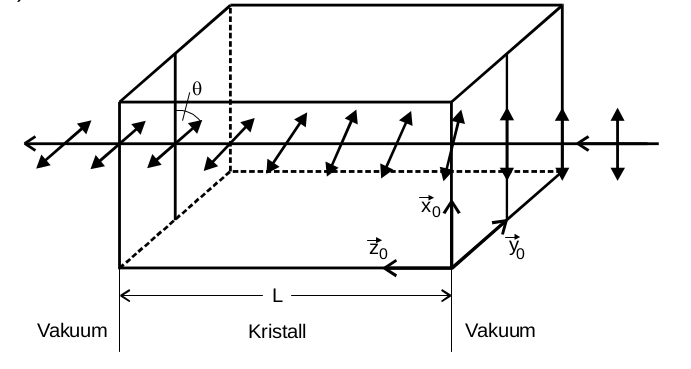
\includegraphics[width=1\textwidth]{pictures/drehung.png}
	         \caption{Drehung der Polarisationsebene einer Lichtwelle beim Durchgang durch einen Kristall \cite{Anleitung}
		 }
		   \label{fig:Bild1}
\end{figure}
Zur Berechnung des Drehwinkels $\theta$ wird der linear polarisierte Lichtstrahl zunächst in einen linkshändigen und einen rechtshändigen Anteil zerlegt:
\begin{equation*}
	E(z)= \frac{1}{2}(E_R(z)+E_L(z)) \, \mathrm{,}
\end{equation*}
wobei sich beide Wellen in z-Richtung fortbewegen und unterschiedliche Wellenzahlen besitzen ($k_R \neq k_L$).
Mit dem Wellenansatz für die beiden Wellen, den beiden Definitionen
\begin{align}\label{Winkel}
	\psi := \frac{L}{2} (k_R + k_L) \\\nonumber
	\theta := \frac{L}{2} (k_R - k_L)
\end{align}
und der Eulerschen Formel folgt:
\begin{align}
	E(L)=E_0 e^{i\psi}(cos(\theta ) \vec{x_o} + sin(\theta ) \vec{y_0} ) \, \mathrm{.}
\end{align}
Der Drehwinkel $\theta$ lässt sich auch durch die Brechungsindizes ausdrücken:
\begin{align*}
	\theta = \frac{L \omega}{2 c} (n_R - n_L) \mathrm{.}
\end{align*}
Für die Polarisation $\vec{P}$ im Kristall, falls nicht zu große Felder betrachtet werden, gilt
\begin{equation*}
	\vec{P}=\varepsilon_0 \chi \vec{E} \, \mathrm{,}
\end{equation*}
mit der dielektrischen Suszeptibilität $\chi$. Da die Materie doppelbrechend ist, gilt für den $\chi$-Tensor:
\begin{equation*}
	\vec{\chi} =
	\begin{pmatrix}
		\chi_{xx} & i\chi_{xy} & 0 \\
		-\chi_{xy} & \chi_{xx} & 0 \\
		0 & 0 & \chi_{zz}a
	\end{pmatrix} \, \mathrm{.}
\end{equation*}
Für die Wellengleichung des Lichtes mit einer dielektrischen Verschiebung $\vec{D}=\varepsilon_0 \vec{E} + \vec{P}$ folgt die Gleichung:
\begin{equation*}
	\nabla \times (\nabla \times \vec{E}) = -\frac{1}{c^2}(1+\chi)\frac{\partial^2\vec{E}}{\partial t^2} \, \mathrm{.}
\end{equation*}
Mit der Paramatrisierung von $\vec{E}$ als ebene Welle folgt ein Gleichungssystem, welches die
Lösung
\begin{equation*}
	k_{\pm} = \frac{\omega}{c}\sqrt{(1+\chi_{xx}) \pm \chi_{xy}}
\end{equation*}
besitzt. Da der Wellenzahlvektor von der Phasengeschwindigkeit abhängt wird nun klar das eine linkszirkluar und eine rechtszirkular polarisierte Welle unterschiedliche Phasengeschwindigkeiten besitzen. So folgt für den Drehwinkel $\theta$ aus Gleichung \eqref{Winkel}:
\begin{equation*}
	\theta \approx \frac{L\omega}{2c}(\sqrt{1+\chi_{xx}})^{-1}\chi_{xy} \approx \frac{L\omega}{2cn}\chi_{xy} \, \mathrm{.}
\end{equation*}
Für ein gebundenes Elektron der Masse $m$ und der Ladung $e_0$ unter dem Einfluss eines elektromagnetischen Feldes wird folgende Gleichung angenommen:
\begin{equation*}
	m\frac{\mathrm{d}^2\vec{r}}{\mathrm{d}t^2}+K\vec{r} = - e_o \vec{E}(r) -e_0 \frac{\mathrm{d}\vec{r}}{\mathrm{d}t}\times \vec{B} \, \mathrm{.}
\end{equation*}
Hieraus folgt nach einigen Rechnungen folgende Formel für den Drehwinkel:
\begin{equation*}
	\theta = \frac{e_0^3}{2 \varepsilon_0 c m^2} \frac{\omega^2}{\left(-\omega^2+\frac{K}{m}
	\right)^2-\left(\frac{e_0}{m}B\omega\right)^2}\frac{NBL}{n} \, \mathrm{.}
\end{equation*}
Mit einigen weiteren Einschränkungen folgt für den Fall von quasifreien Ladungsträgern:
\begin{equation}\label{eqn:Masse}
	\theta_{frei}\approx\frac{e_0^3}{8 \pi^2 \varepsilon_0 c^3 m^2}\lambda^2\frac{NBL}{n} \, \mathrm{.}
\end{equation}
